% Options for packages loaded elsewhere
\PassOptionsToPackage{unicode}{hyperref}
\PassOptionsToPackage{hyphens}{url}
\PassOptionsToPackage{dvipsnames,svgnames*,x11names*}{xcolor}
%
\documentclass[
  12pt,
]{article}
\usepackage{lmodern}
\usepackage{amssymb,amsmath}
\usepackage{ifxetex,ifluatex}
\ifnum 0\ifxetex 1\fi\ifluatex 1\fi=0 % if pdftex
  \usepackage[T1]{fontenc}
  \usepackage[utf8]{inputenc}
  \usepackage{textcomp} % provide euro and other symbols
\else % if luatex or xetex
  \usepackage{unicode-math}
  \defaultfontfeatures{Scale=MatchLowercase}
  \defaultfontfeatures[\rmfamily]{Ligatures=TeX,Scale=1}
\fi
% Use upquote if available, for straight quotes in verbatim environments
\IfFileExists{upquote.sty}{\usepackage{upquote}}{}
\IfFileExists{microtype.sty}{% use microtype if available
  \usepackage[]{microtype}
  \UseMicrotypeSet[protrusion]{basicmath} % disable protrusion for tt fonts
}{}
\makeatletter
\@ifundefined{KOMAClassName}{% if non-KOMA class
  \IfFileExists{parskip.sty}{%
    \usepackage{parskip}
  }{% else
    \setlength{\parindent}{0pt}
    \setlength{\parskip}{6pt plus 2pt minus 1pt}}
}{% if KOMA class
  \KOMAoptions{parskip=half}}
\makeatother
\usepackage{xcolor}
\IfFileExists{xurl.sty}{\usepackage{xurl}}{} % add URL line breaks if available
\IfFileExists{bookmark.sty}{\usepackage{bookmark}}{\usepackage{hyperref}}
\hypersetup{
  pdftitle={Text Mining},
  pdfauthor={Eyayaw Teka Beze},
  colorlinks=true,
  linkcolor=teal,
  filecolor=Maroon,
  citecolor=Blue,
  urlcolor=blue,
  pdfcreator={LaTeX via pandoc}}
\urlstyle{same} % disable monospaced font for URLs
\usepackage[margin=1in]{geometry}
\usepackage{longtable,booktabs}
% Correct order of tables after \paragraph or \subparagraph
\usepackage{etoolbox}
\makeatletter
\patchcmd\longtable{\par}{\if@noskipsec\mbox{}\fi\par}{}{}
\makeatother
% Allow footnotes in longtable head/foot
\IfFileExists{footnotehyper.sty}{\usepackage{footnotehyper}}{\usepackage{footnote}}
\makesavenoteenv{longtable}
\usepackage{graphicx,grffile}
\makeatletter
\def\maxwidth{\ifdim\Gin@nat@width>\linewidth\linewidth\else\Gin@nat@width\fi}
\def\maxheight{\ifdim\Gin@nat@height>\textheight\textheight\else\Gin@nat@height\fi}
\makeatother
% Scale images if necessary, so that they will not overflow the page
% margins by default, and it is still possible to overwrite the defaults
% using explicit options in \includegraphics[width, height, ...]{}
\setkeys{Gin}{width=\maxwidth,height=\maxheight,keepaspectratio}
% Set default figure placement to htbp
\makeatletter
\def\fps@figure{htbp}
\makeatother
\setlength{\emergencystretch}{3em} % prevent overfull lines
\providecommand{\tightlist}{%
  \setlength{\itemsep}{0pt}\setlength{\parskip}{0pt}}
\setcounter{secnumdepth}{5}
\usepackage{booktabs}
\usepackage{longtable}
\usepackage{array}
\usepackage{multirow}
\usepackage{wrapfig}
\usepackage{float}
\usepackage{colortbl}
\usepackage{pdflscape}
\usepackage{tabu}
\usepackage{threeparttable}
\usepackage{threeparttablex}
\usepackage[normalem]{ulem}
\usepackage{makecell}
\usepackage{xcolor}

\title{Text Mining}
\usepackage{etoolbox}
\makeatletter
\providecommand{\subtitle}[1]{% add subtitle to \maketitle
  \apptocmd{\@title}{\par {\large #1 \par}}{}{}
}
\makeatother
\subtitle{Text analysis of Chinese Paper Daily news article}
\author{Eyayaw Teka Beze}
\date{2020-04-07}

\begin{document}
\maketitle

{
\hypersetup{linkcolor=}
\setcounter{tocdepth}{2}
\tableofcontents
}
\hypertarget{description-of-data}{%
\section{Description of Data}\label{description-of-data}}

The data are collected from the Chinese \href{https://en.wikipedia.org/wiki/People\%27s_Daily}{People's Daily} newspaper for year 2019 and 2020. The daily newspapers are published on a consistent structure (we give the details of the structure below) online on the newspaper's \href{paper.people.com.cn}{website}. Despite the slow loading speed of the website, We tapped into its structure and have scraped the \textbf{first two pages} of the daily newspapers.

For instance, the 1st page of the issue published on \emph{2020-03-22} can be accessed \href{http://paper.people.com.cn/rmrb/html/2020-03/22/nbs.D110000renmrb_01.htm}{here}.

\hypertarget{r-example-newspaper-resultsh-out.width49-out.height20fig.showhold-fig.aligncenter-fig.capexample-newspaper-page-published-on-2020-03-22-left-and-section-or-column-1-of-it-enlarged-right.-include_graphicsc-herefigsexample_newspaper_page.pdf-herefigssection1_enlarged.pdf-dpi-na}{%
\section{\texorpdfstring{\texttt{\{r,\ example-newspaper,\ results="H",\ out.width="49\%",\ out.height="20\%",fig.show=\textquotesingle{}hold\textquotesingle{},\ fig.align=\textquotesingle{}center\textquotesingle{},\ fig.cap="Example\ newspaper\ page\ published\ on\ 2020-03-22\ (left),\ and\ Section\ or\ column\ 1\ of\ it\ enlarged\ (right)."\}\ \#\ \ \#\ include\_graphics(c(\ \#\ \ \ here("figs/example\_newspaper\_page.pdf"),\ \#\ \ \ here("figs/section1\_enlarged.pdf")\ \#\ ),\ dpi\ =\ NA)\ \#}}{\{r, example-newspaper, results="H", out.width="49\%", out.height="20\%",fig.show='hold', fig.align='center', fig.cap="Example newspaper page published on 2020-03-22 (left), and Section or column 1 of it enlarged (right)."\} \#  \# include\_graphics(c( \#   here("figs/example\_newspaper\_page.pdf"), \#   here("figs/section1\_enlarged.pdf") \# ), dpi = NA) \#}}\label{r-example-newspaper-resultsh-out.width49-out.height20fig.showhold-fig.aligncenter-fig.capexample-newspaper-page-published-on-2020-03-22-left-and-section-or-column-1-of-it-enlarged-right.-include_graphicsc-herefigsexample_newspaper_page.pdf-herefigssection1_enlarged.pdf-dpi-na}}

We dissect the different characteristics of this particular article as follows and these properties apply to all other articles.

First of all, the main link to the article is this one: (\url{http://paper.people.com.cn/rmrb/html/2020-03/22/nbs.D110000renmrb_01.htm}). This takes us to one page of the newspaper, i.e., to the 1st page of the newspaper in this particular example. However, a lot of content is packed on this single page. There are 10 different sections or columns on this article (see Figure \ref{fig:example-newspaper} for this example newspaper page published on 2020-03-22).

\begin{itemize}
\item
  The prefix of the URL, i.e.,
  \textbf{(\url{http://paper.people.com.cn/rmrb/html})} is the same for every article, regardless of page number or edition.
\item
  Date on which it was published: \textbf{2020-03/22}
\item
  Page number of the newspaper: \textbf{01}
\item
  Section id prefix: \textbf{nbs.D110000renmrb}.
\end{itemize}

As we can see in Figure (\ref{fig:example-newspaper}) there are several different sections crammed or squeezed into the single page of the newspaper and these parts (sections) are clickable, and each has a unique id. A click on each section will redirect to a link where one can access the full content of the section in an enlarged view. For example, the first section out of the 10 sections on this example article is \href{http://paper.people.com.cn/rmrb/html/2020-03/22/nw.D110000renmrb_20200322_1-01.htm}{section 1} or (see Figure \ref{fig:example-newspaper} --right). The section id for this first section is \textbf{nw.D110000renmrb\_20200322\_1-01}.

Accordingly, the id of each section on an article is of this form:
\textbf{nw.D110000renmrb\_yyyymmdd\_section\#-page\#}. Each section of the single page newspaper has the following additional characteristics.

\begin{itemize}
\tightlist
\item
  Title (\textbf{h1 tag})
\item
  Subtitle (\textbf{h3 tag})
\item
  Number of paragraphs on each page, and
\item
  Content or body of the news article section.
\end{itemize}

The maximum number of sections on a page is 15, in \href{http://paper.people.com.cn/rmrb/html/2019-04/26/nbs.D110000renmrb_01.htm}{an article published on 2019-04-26}, and the minimum is 1. On average, there were 5.99 sections per a page of an article, for the newspapers published since January 1st, 2019 regardless of the page number. Looking at the frequencies of articles individually, the tendency is for page 2 to have less issues with very high numbers of articles above around 9.

\textbackslash begin\{figure\}

\{\centering 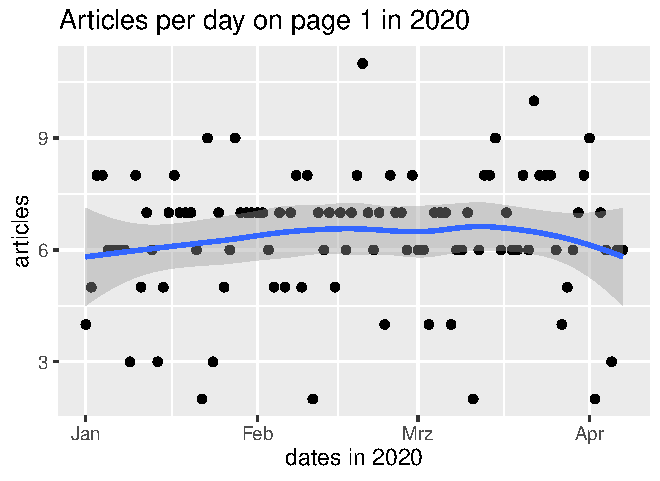
\includegraphics[width=0.49\linewidth,height=0.2\textheight]{C:/Users/David/Seafile/Meine Bibliothek/Kurse/adv-r/Advanced_R_Project/figs/art_freq201} 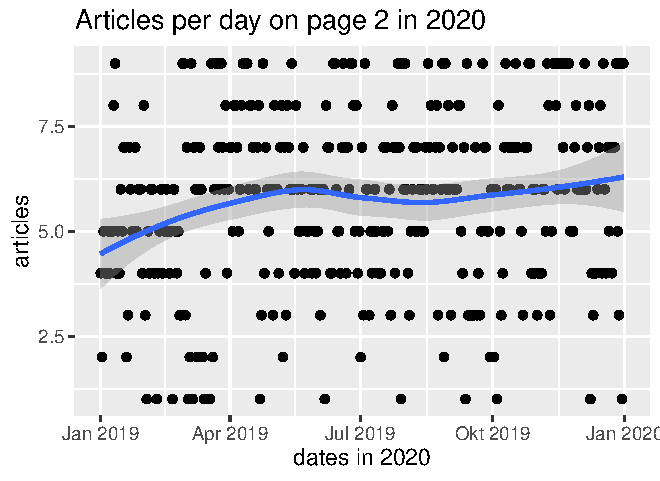
\includegraphics[width=0.49\linewidth,height=0.2\textheight]{C:/Users/David/Seafile/Meine Bibliothek/Kurse/adv-r/Advanced_R_Project/figs/art_freq202}

\}

\caption{Articles per day for page 1 and page 2.}

(\#fig:art\_frequencies)
\textbackslash end\{figure\}

Therefore, the contents of all the sections together--on the page of the news article-- make up the contents of the entire (single) page--which are compactly placed in a single page of the article. Particularly, we scraped the sections of the newspapers--through their unique ids. The date and the page number of the newspaper uniquely identify a newspaper, where the combination of which forms the ids of the sections--prefixed with \textbf{nbs.D110000renmrb}.

Moreover, most of the news articles are bulky in terms of number of paragraphs and text volume. There are 82.67 number of paragraphs per page, and 16.6

\hypertarget{descriptive-statistics}{%
\section{Descriptive Statistics}\label{descriptive-statistics}}

\begin{table}

\caption{\label{tab:desc-stat-table}Descriptive Statistics: How bulky is the daily newspaper?}
\centering
\resizebox{\linewidth}{!}{
\begin{tabular}[t]{lrrrrrrrrrr}
\toprule
\multicolumn{1}{c}{\em{\textbf{}}} & \multicolumn{5}{c}{\em{\textbf{Page 1}}} & \multicolumn{5}{c}{\em{\textbf{Page 2}}} \\
\cmidrule(l{3pt}r{3pt}){2-6} \cmidrule(l{3pt}r{3pt}){7-11}
Variable & median & mean & sd & max & min & median & mean & sd & max & min\\
\midrule
\rowcolor{gray!6}  \addlinespace[0.3em]
\multicolumn{11}{l}{\textit{\textbf{2019}}}\\
\hspace{1em}num\_of\_paragraphs & 77.0 & 91.9 & 55.8 & 367.0 & 20.0 & 70.0 & 76.6 & 30.5 & 246 & 9.0\\
\hspace{1em}num\_of\_sections & 6.0 & 6.2 & 1.8 & 15.0 & 1.0 & 6.0 & 5.7 & 2.1 & 9 & 1.0\\
\rowcolor{gray!6}  \hspace{1em}paragraph\_per\_section & 12.7 & 15.6 & 9.4 & 65.5 & 4.1 & 12.7 & 18.5 & 23.5 & 246 & 4.2\\
\hspace{1em}words & 2898.0 & 3326.3 & 1756.0 & 16190.0 & 803.0 & 2537.0 & 2661.3 & 888.1 & 8675 & 219.0\\
\rowcolor{gray!6}  \addlinespace[0.3em]
\multicolumn{11}{l}{\textit{\textbf{2020}}}\\
\hspace{1em}num\_of\_paragraphs & 69.0 & 83.4 & 48.5 & 341.0 & 30.0 & 66.0 & 70.0 & 26.5 & 204 & 9.0\\
\hspace{1em}num\_of\_sections & 7.0 & 6.4 & 1.7 & 11.0 & 2.0 & 6.0 & 6.0 & 2.0 & 9 & 1.0\\
\rowcolor{gray!6}  \hspace{1em}paragraph\_per\_section & 11.3 & 14.0 & 8.9 & 56.8 & 4.2 & 10.0 & 15.7 & 22.4 & 204 & 4.0\\
\hspace{1em}words & 2871.0 & 3135.8 & 1218.8 & 9732.0 & 1508.0 & 2444.0 & 2439.9 & 643.3 & 4270 & 232.0\\
\bottomrule
\end{tabular}}
\end{table}

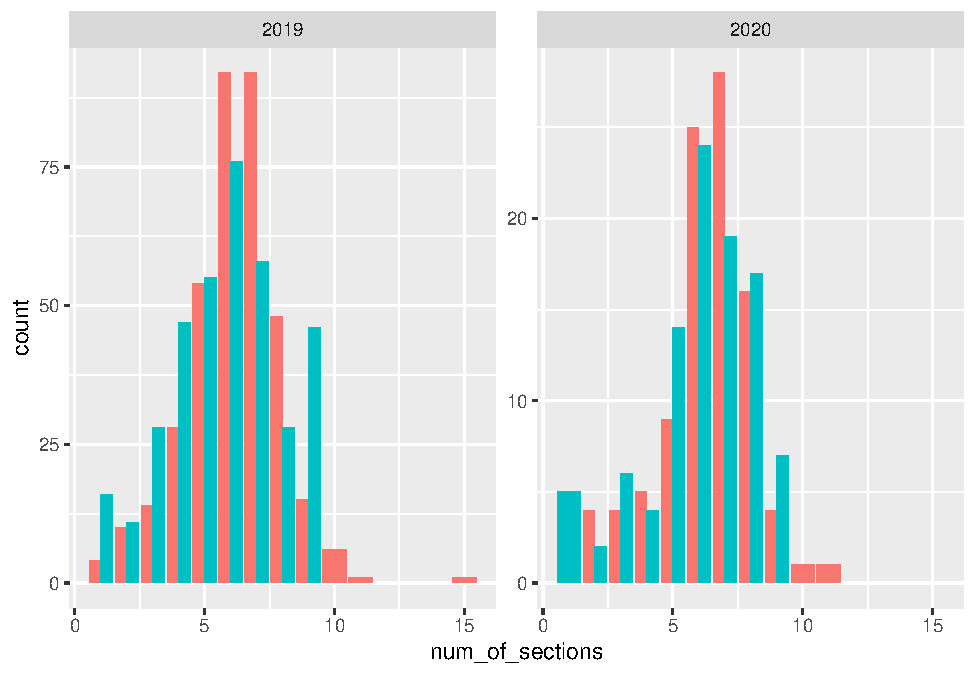
\includegraphics{text_analysis_files/figure-latex/plotting-1.pdf} 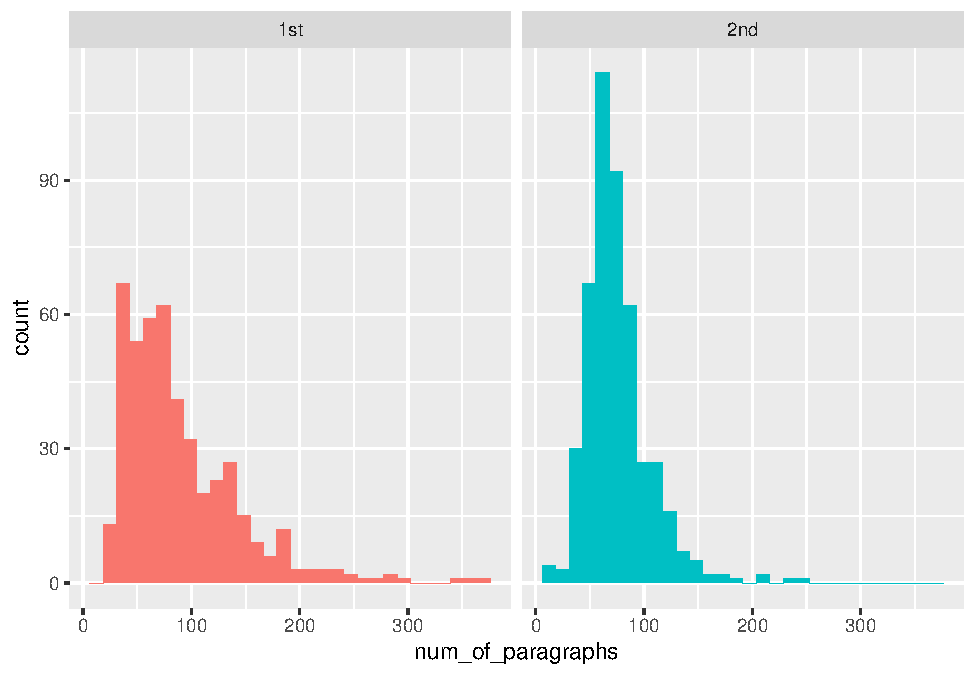
\includegraphics{text_analysis_files/figure-latex/plotting-2.pdf} 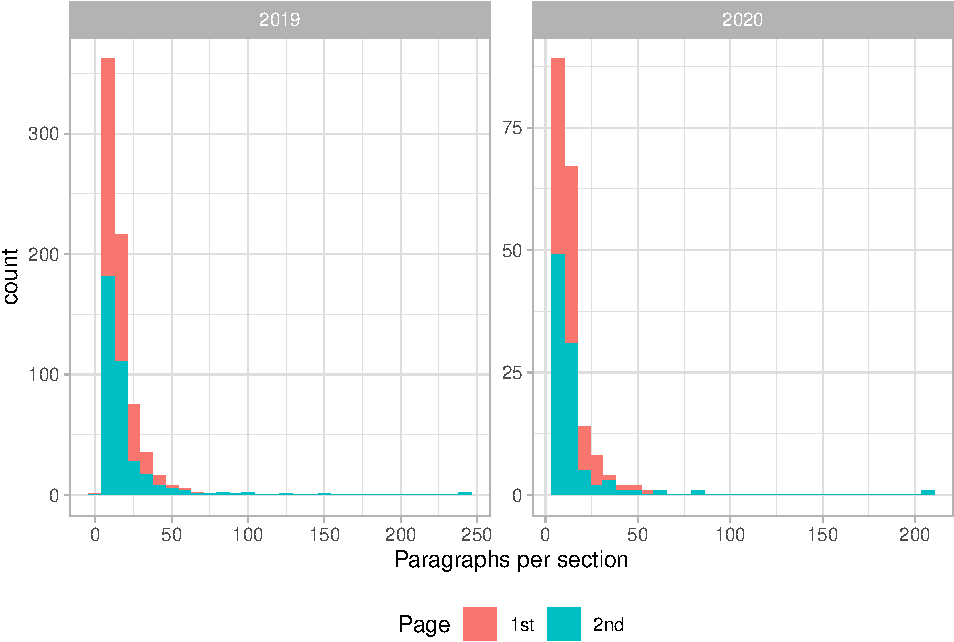
\includegraphics{text_analysis_files/figure-latex/plotting-3.pdf} 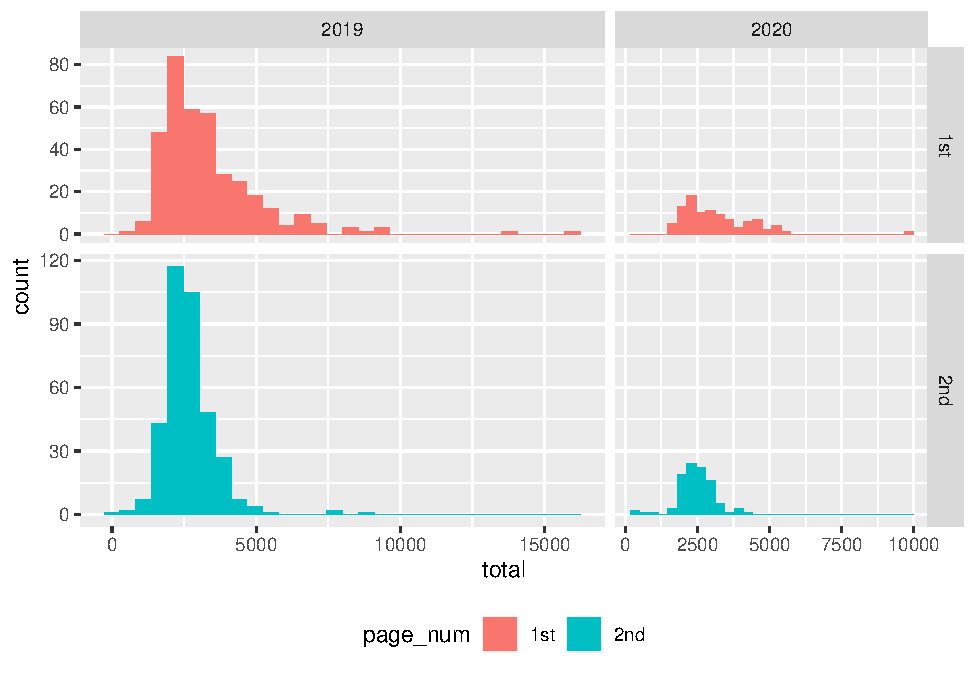
\includegraphics{text_analysis_files/figure-latex/plotting-4.pdf}

\begin{figure}
\centering
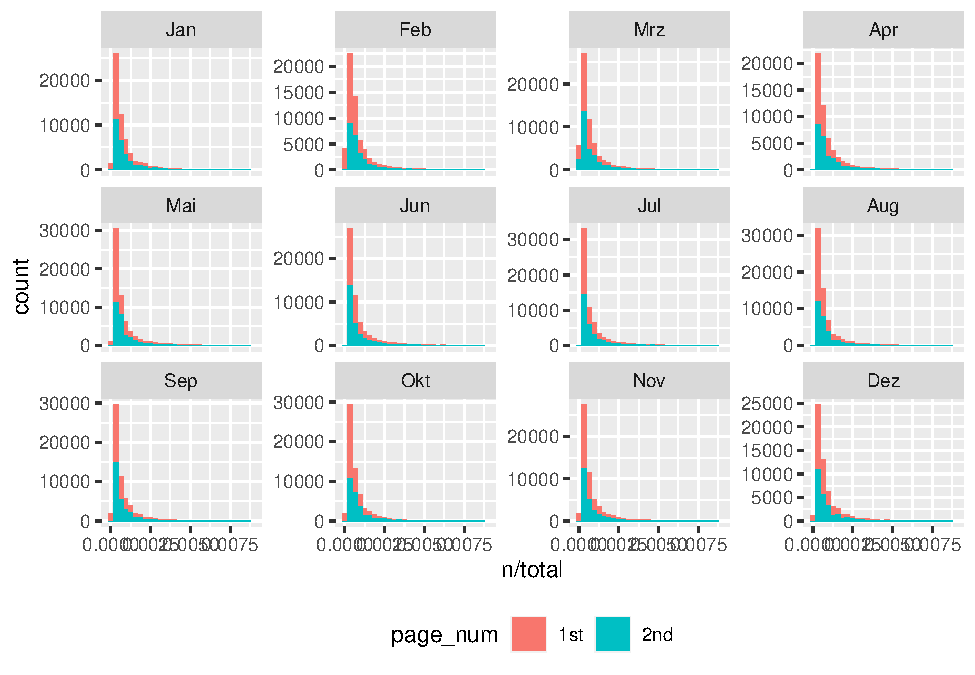
\includegraphics{text_analysis_files/figure-latex/unnamed-chunk-2-1.pdf}
\caption{\label{fig:unnamed-chunk-2}term frequency common words}
\end{figure}

\end{document}
